%%%%%%%%%%%%%%%%%%%%%%% file typeinst.tex %%%%%%%%%%%%%%%%%%%%%%%%%
%
% This is the LaTeX source for the instructions to authors using
% the LaTeX document class 'llncs.cls' for contributions to
% the Lecture Notes in Computer Sciences series.
% http://www.springer.com/lncs       Springer Heidelberg 2006/05/04
%
% It may be used as a template for your own input - copy it
% to a new file with a new name and use it as the basis
% for your article.
%
% NB: the document class 'llncs' has its own and detailed documentation, see
% ftp://ftp.springer.de/data/pubftp/pub/tex/latex/llncs/latex2e/llncsdoc.pdf
%
%%%%%%%%%%%%%%%%%%%%%%%%%%%%%%%%%%%%%%%%%%%%%%%%%%%%%%%%%%%%%%%%%%%


\documentclass[runningheads,a4paper]{article}

\setcounter{tocdepth}{3}
\usepackage{graphicx}
% For citations
\usepackage{natbib}
\usepackage{amsmath,amsfonts,amscd,amssymb}
\usepackage{dsfont}
\renewcommand{\vec}[1]{\mathbf{#1}}
\usepackage{hyperref}
\DeclareMathOperator*{\argmax}{argmax}
\DeclareMathOperator*{\argmin}{argmin}
\DeclareMathOperator*{\Corr}{Corr}
\newcommand{\R}{\mathds{R}}
\usepackage{multicol}
\usepackage{multirow}
\usepackage{pbox}
\usepackage{url}
\urldef{\mailsa}\path|{felix.biessmann,|
\newcommand{\keywords}[1]{\par\addvspace\baselineskip
\noindent\keywordname\enspace\ignorespaces#1}

\begin{document}

 % start of an individual contribution

% first the title is needed
\title{Speeding up the manifesto project: Active learning strategies for efficient automated political annotations}

% a short form should be given in case it is too long for the running head
\title{Speeding up the manifesto project: \\ Active learning strategies for \\efficient automated political annotations}

% the name(s) of the author(s) follow(s) next
%
% NB: Chinese authors should write their first names(s) in front of
% their surnames. This ensures that the names appear correctly in
% the running heads and the author index.
%
\author{
%Felix Biessmann\thanks{felix.biessmann@gmail.com},~ 
%Philipp Schmidt\thanks{schmidtiphil@gmail.com}, ~ 
%Andreas Grafberger\thanks{}
}
%
%\authorrunning{Active Learning for Political Annotations}}
% (feature abused for this document to repeat the title also on left hand pages)

% the affiliations are given next; don't give your e-mail address
% unless you accept that it will be published
%\institute{
%\mailsa\\
%\mailsb\\
%\mailsc\\
%\url{http://www.springer.com/lncs}}

%
% NB: a more complex sample for affiliations and the mapping to the
% corresponding authors can be found in the file "llncs.dem"
% (search for the string "\mainmatter" where a contribution starts).
% "llncs.dem" accompanies the document class "llncs.cls".
%

%\toctitle{}
%\tocauthor{}
\maketitle

\begin{abstract} 
The Manifestoproject Corpus is an exceptional data source for political education as it combines political texts with valuable annotations by human experts. However the amount of data human annotators can label is very limited compared to the ever increasing amount of political texts published in manifestos, news media and social networks. The discrepancy between labeling budget and data that needs to be labelled highlights the necessity of automated annotations by means of machine learning (ML). Taking into account label consistency across human experts, which is often not perfect and thus requires to collect at least three labels per data point, this discrepancy is even worse. 

When only a small fraction of the available data can be labelled in order to train an ML model, the priority of which samples should be labelled first is important: Some samples are easy to classify - those should not be labelled with high priority, as the classifier will not learn much from them. For these samples it is relatively safe to have them labelled automatically by an ML model without wasting the time of human annotators. Other data points are difficult for the ML model; when labels for those are obtained first, the model will reach its optimal classification performance faster. 

In this study we leverage this insight, known in the ML community as active learning. We present offline experiments on the manifesto corpus showing that active learning strategies significantly speed up training of ML models for manifesto code annotations. This shows the potential of ML methods as assistive technology for political science. To demonstrate the benefits of this approach we present an implementation of a web based active learning annotation system that can be readily used for speeding up the manifesto annotations as well as annotations of other political texts.
\end{abstract} 

\section{Introduction}
\label{sec:intro}
%

\section{Results}
\label{sec:results}
Basically: it works, see also \autoref{fig:active_learning_curves}.
\begin{figure}
\begin{center}
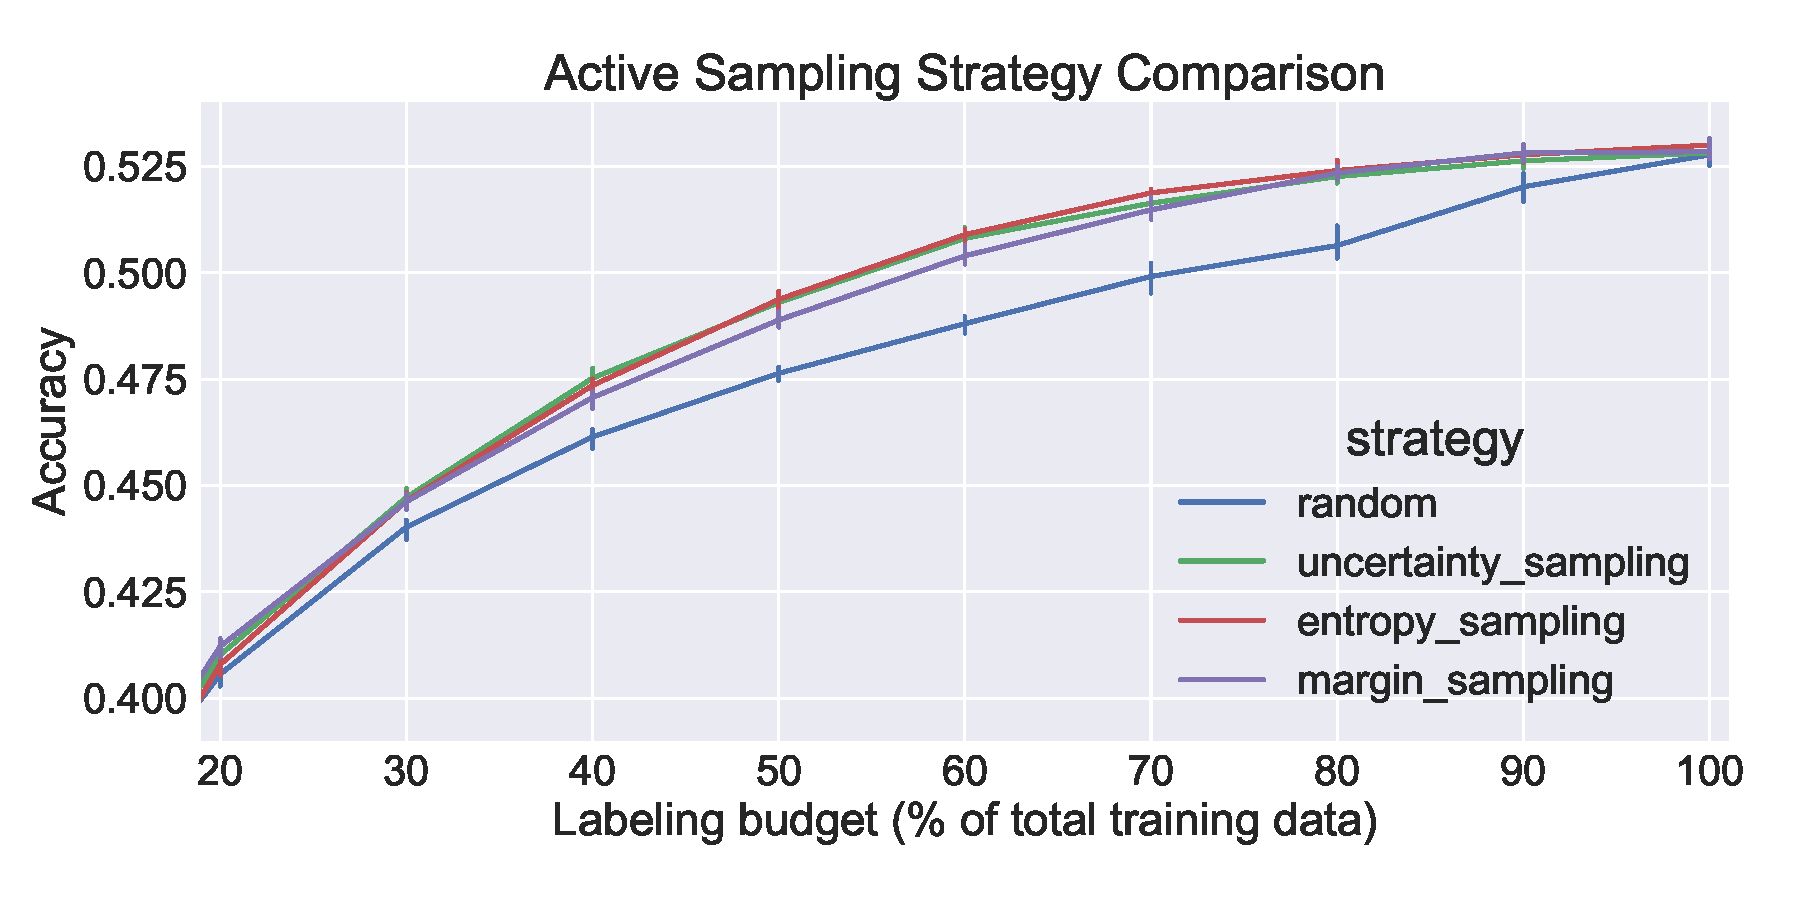
\includegraphics[width=0.9\textwidth]{images/active_learning_manifesto.pdf} 
%
\end{center}
\caption{
\label{fig:active_learning_curves}
}
\end{figure}


%\section{Data Sets and Feature Extraction}\label{sec:data}
%%
%
%\subsection{Data}
%Annotated political text data was obtained from two sources: a) the discussions and speeches held in the german parliament ({\em Bundestag}) and b) all manifesto texts of parties running for election in the german parliament in the current 18th and the last, 17th, legislation period.
%
%\paragraph{Parliament discussion data} Parliament texts are annotated with the respective party label, which we take here as a proxy for political bias. The texts of parliament protocols are available through the website of the german bundestag\footnote{\url{https://www.bundestag.de/protokolle}}; an open source API was used to query the data in a cleaned and structured format\footnote{\url{https://github.com/bundestag}}. In total 22784 speeches were extracted for the 17th legislative period and 11317 speeches for the 18th period, queried until March 2016. 
%
%\paragraph{Party manifesto data}
%For party manifestos another openly accessible API was used, provided by the Wissenschaftszentrum Berlin (WZB). The API is released as part of the {\em Manifestoproject} \cite{manifesto}. The data released in this project comprises the complete manifestos for each party that ran for election enriched with annotations by political experts. Each sentence (in some cases also parts of sentences) is annotated with one of 56 political labels. Examples of these labels are {\em pro/contra protectionism, decentralism, centralism, pro/contra welfare}; for a complete list and detailed explanations on how the annotators were instructed see \cite{leftright}. The set of labels was developed by political scientists at the WZB and released for public use. All manifestos of parties that were running for election in this and the last legislative period were obtained. In total this resulted in 29451 political statements that had two types of labels: First the party affiliation of each political statement; this label was used to evaluate the party evaluation classifiers trained on the parliament speeches. For this purpose the data acquisition was constrained to only those parties that were elected into the parliament. Next to the party affiliation the political view labels were extracted. For the analyses based on political view labels all parties were considered, also those that did not make it into the parliament. 
%
%The length of each annotated statement in the party manifestos was rather short. The longest statement was 522 characters long, the 25\%/50\%/75\% percentiles were 63/95/135 characters. Measured in words the longest data point was 65 words and the 25\%/50\%/75\% percentiles were 8/12/17 words, respectively. This can be considered as a very valuable property of the data set, because it allows a fine grained resolution of party manifestos. However for a classifier (as well as for humans) such short sentences can be rather difficult to classify. In order to obtain less 'noisy' data points from each party -- for the party affiliation task only -- all statements were aggregated into political topics using the manifesto code labels. Each political view label is a three digit code, the first digit represents the political domain. In total there were eight political domains (topics): {\em External Relations, Freedom and Democracy, Political System, Economy, Welfare and Quality of Life, Fabric of Society, Social Groups} and a topic {\em undefined}, for a complete list see also \cite{leftright}. These 8 topics were used to aggregate all statements in each manifesto into topics. Most party manifestos covered all eight of them, some party manifestos in the 17th Bundestag only covered seven. 
%
%\subsection{Bag-of-Words Vectorization}\label{sec:bow-vectorization}
%First each data set was segmented into semantic units; in the case of parliament discussions this were the speeches, in the case of the party manifesto data semantic units were the sentences or sentence parts associated with one of the 56 political view labels.  Parliament speeches were often interrupted; in this case each uninterrupted part of a speech was considered a semantic unit. Strings of each semantic unit were tokenised and transformed into bag-of-word vectors as implemented in scikit-learn \cite{scikit-learn}. The general idea of bag-of-words vectors is to simply count occurrences of words (or word sequences, also called {\em n-grams}) for each data point. A data point is usually a document, here it is the semantic units of parliament speeches and manifesto sentences, respectively. The text of each semantic unit is transformed into a vector $\vec{x}\in\mathds{R}^d$ where $d$ is the size of the dictionary; the $w$th entry of $\vec{x}$ contains the (normalized) count of the $w$th word (or sequence of words) in our dictionary. Several options for vectorizing the speeches were tried, including term-frequency-inverse-document-frequency normalisation, n-gram patterns up to size $n=3$ and several cutoffs for discarding too frequent and too infrequent words. All of these hyperparameters were subjected to hyperparameter optimization as explained in \autoref{sec:crossvalidation}. 
%
%
%\section{Classification Model and Training Procedure}\label{sec:model}
%Bag-of-words feature vectors were used to train a multinomial logistic regression model. Let $y\in\{1,2,\dots,K\}$ be the true  label, where $K$ is the total number of labels and $\vec{W}=[\vec{w}_1,\dots,\vec{w}_K]\in\R^{d\times K}$ is the concatenation of the weight vectors $\vec{w}_k$ associated with the $k$th party then 
%\begin{eqnarray}\label{eq:logreg_multiclass}
%p(y=k|\vec{x},\vec{W}) = &\frac{e^{z_k}}{\sum_{j=1}^K e^{z_j}} \qquad \textrm{with }  z_k=&\vec{w}_k^{\top}\vec{x} \\\nonumber
%\end{eqnarray}
%%
%We estimated $\vec{W}$ using quasi-newton gradient descent. The optimization function was obtained by adding a penalization term to the negative log-likelihood of the multinomial logistic regression objective and the optimization hence found the $\vec{W}$ that minimized
%\begin{equation}\label{eq:objective}
%L(\vec{W}, \vec{x}, \gamma) = - \log{\frac{e^{z_k}}{\sum_{j=1}^K e^{z_j}}}+ \gamma \| \vec{W} \|_{F}
%\end{equation}
%Where $\|~\|_F$ denotes the Frobenius Norm and $\gamma$ is a regularization parameter controlling the complexity of the model. 
%The regularization parameter was optimized on a log-scaled grid from $10^{-4,\dots,4}$. The performance of the model was optimized using the classification accuracy, but we also report all other standard measures, precision ($TP / (FP + TP$), recall ($TP / (TP + FN)$) and f1-score ($2\times (Prec. \times Rec) / (Prec + Rec.)$). \\
%
%Three different classification problems were considered: 
%\begin{enumerate}
%\item {\bf Classification of party affiliation} (five class / four class problem)
%\item {\bf Classification of government membership} (binary problem)
%\item {\bf Classification of political views} (56 class problem)
%\end{enumerate}
%
%Party affiliation is a five class problem for the 17th legislation period, and a four class problem for the 18th legislation period. Political view classification is based on the labels of the manifesto project, see \autoref{sec:data} and \cite{leftright}. 
%For each of first two problems, party affiliation and government membership prediction, classifiers were trained on the parliament speeches. For the third problem classifiers were trained only on the manifesto data for which political view labels were available. 
%
%\subsection{Optimisation of Model Parameters}\label{sec:crossvalidation}
%The model pipeline contained a number of  hyperparameters that were optimised using cross-validation.  
%We first split the training data into a training data set that was used for optimisation of hyperparameters and an held-out test data set for evaluating how well the model performs on in-domain data; wherever possible the generalisation performance of the models was also evaluated on out-of domain data. Hyperparameters were optimised using grid search and 3-fold cross-validation within the training set only: A cross-validation split was made to obtain train/test data for the grid search and for each setting of hyperparameters the entire pipeline was trained and evaluated -- no data from the in-domain evaluation data or the out-of-domain evaluation data were used for hyperparameter optimisation. For the best setting of all hyperparameters the pipeline was trained again on all training data and evaluated on the evaluation data sets. For party affiliation prediction and government membership prediction the training and test set were 90\% and 10\%, respectively, of all data in a given legislative period. Out-of-domain evaluation data were the texts from party manifestos. For the political view prediction setting there was no out-of-domain evaluation data, so all labeled manifesto sentences in both legislative periods were split into a training and evaluation set of 90\% (train) and 10\% (evaluation). 

\subsection*{Acknowledgements}

%
\small{
\bibliographystyle{plain}
\bibliography{political_bias_prediction} 
}


\end{document}